\documentclass[10pt]{beamer}
\usetheme{Madrid}
\usecolortheme{beaver}
\usepackage{tikz}
\usetikzlibrary{automata, positioning, arrows}

\title[Sequence Detector]
{Sequence Detector}
\subtitle{DCS Final Presentation}
\institute{DTU}
\author{Jatin Pandey \& kumood}
\logo{
  \includegraphics[height=1cm]{./src/logo.png}
}
\begin{document}
  \frame {
      \titlepage
    }
  \frame {
      \frametitle{What is a Sequence Detector?}
      A sequence detector accepts as input a string of bits: either 0 or 1.   Its output goes to 1 when a target sequence has been detected.
    }
  \frame{
      \frametitle{Types of Sequence Detector}
      There are two basic types of Sequence Detector
      \begin{itemize}
        \item Overlap
        \item Non-Overlap
      \end{itemize}
    }
  \frame{
      \frametitle{Simple Finite State Machine}
    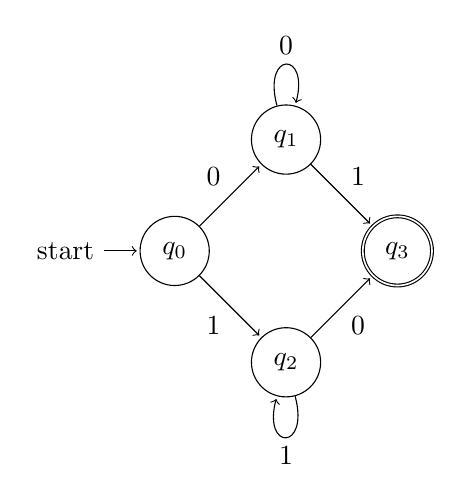
\begin{tikzpicture}[shorten >=1pt,node distance=2cm,on grid,auto] 
     \node[state,initial] (q_0)   {$q_0$}; 
      \node[state] (q_1) [above right=of q_0] {$q_1$}; 
     \node[state] (q_2) [below right=of q_0] {$q_2$}; 
      \node[state,accepting](q_3) [below right=of q_1] {$q_3$};
      \path[->] 
      (q_0) edge  node {0} (q_1)
      edge  node [swap] {1} (q_2)
      (q_1) edge  node  {1} (q_3)
      edge [loop above] node {0} ()
      (q_2) edge  node [swap] {0} (q_3) 
      edge [loop below] node {1} ();
    \end{tikzpicture}
    }
\end{document}
